
\documentclass[letter]{article}
\usepackage{a4wide}
\setlength{\topmargin}{0cm}
\setlength{\topskip}{0cm}
\setlength{\headsep}{0cm}
\usepackage{amstext}
\usepackage{amsfonts}
\usepackage{Sweave}
\usepackage{hyperref}
\usepackage{natbib}

\setkeys{Gin}{width=0.727\textwidth}

\usepackage{hyperref}
%% \usepackage[nolists]{endfloat}

\input{head}

\hypersetup{%
  pdftitle = {Unbiased Recursive Partitioning: 
              A Conditional Inference Framework},
  pdfsubject = {Manuscript},   
  pdfauthor = {Anonymous},
%% change colorlinks to false for pretty printing
  colorlinks = {true},  
  linkcolor = {blue},   
  citecolor = {blue},   
  urlcolor = {red},   
  hyperindex = {true},
  linktocpage = {true},
}

\renewcommand{\baselinestretch}{1.78}
%%\setlength{\parindent}{0cm}
%%\setlength{\parskip}{0.5ex}

\renewcommand{\refname}{REFERENCES}

\begin{document}

\title{Unbiased Recursive Partitioning: \\ A Conditional Inference Framework}

\author{Torsten Hothorn$^1$, Kurt Hornik$^2$ and Achim Zeileis$^2$}

\date{Final Version, \today}

\maketitle

\noindent
$^1$ Institut f\"ur Medizininformatik, Biometrie und Epidemiologie\\
     Friedrich-Alexander-Universit\"at Erlangen-N\"urnberg\\
     Waldstra{\ss}e 6, D-91054 Erlangen, Germany \\
     \texttt{Torsten.Hothorn@rzmail.uni-erlangen.de}

\noindent
$^2$ Department f\"ur Statistik und Mathematik, Wirtschaftsuniversit\"at Wien \\
     Augasse 2-6, A-1090 Wien, Austria


\begin{abstract}

Recursive binary partitioning is a popular tool for %% explanatory
regression analysis. Two fundamental problems of exhaustive
search procedures usually applied to fit such models
have been known for a long time: overfitting and a selection bias towards
covariates with many possible splits or missing values. While pruning
procedures are able to solve the overfitting problem, the variable selection
bias still seriously affects the interpretability of tree-structured 
regression models. For some special cases unbiased procedures have been suggested,
however lacking a common theoretical foundation. We propose a unified
framework for recursive partitioning which embeds tree-structured regression
models into a well defined theory of conditional inference procedures.
Stopping criteria based on multiple test procedures are implemented and it is
shown that the predictive performance of the resulting trees is as good as
the performance of established exhaustive search procedures. It turns out
that the partitions and therefore the models induced by both approaches are
structurally different, confirming the need for an unbiased variable
selection. Moreover, it is shown that the prediction accuracy of trees with
early stopping is equivalent to the prediction accuracy of 
pruned trees with unbiased variable selection.
The methodology presented here is applicable to all kinds of regression
problems, including nominal, ordinal, numeric, censored as well as
multivariate response variables and arbitrary measurement scales of the
covariates. Data from studies on glaucoma classification,
node positive breast cancer survival and mammography experience are re-analyzed.


{\bf Key Words:} permutation tests; variable selection; multiple testing; 
                 ordinal regression trees; multivariate regression trees.
\end{abstract}


\begin{center}
\section{INTRODUCTION}
\end{center}

Statistical models that regress the distribution of a response variable
on the status of multiple covariates are tools for handling two major
problems in applied research:
prediction and explanation. The function space represented by
regression models
focusing on the prediction problem may be arbitrarily complex; indeed, 
`black
box' systems like support vector machines or ensemble methods are excellent
predictors. In contrast, regression models appropriate for gaining insight
into the
mechanism of the data generating process are required to offer
a human readable representation. Generalized linear models or
the Cox model are representatives of regression models where 
parameter estimates of the coefficients and their distribution
are used to judge the relevance of single covariates.

With their seminal work on automated interaction detection (AID),
\cite{MorganSonquist1963} introduced another class of simple  
regression models for prediction and explanation 
nowadays known as `recursive partitioning' or `trees'.
Many variants and extensions have been published in the last $40$
years, the majority of which are special cases of a simple two-stage 
algorithm: 
first partition the observations by univariate splits in a recursive way and 
second fit a constant model in each cell of the resulting partition. 
The most popular implementations of such algorithms are `CART' 
\citep{classifica:1984} and `C4.5' \citep{Quinlan1993}. Not unlike AID, 
both perform an exhaustive search over all possible splits maximizing an
information measure of node impurity selecting the 
covariate showing the best split.
This approach has two fundamental problems: overfitting and a selection 
bias towards covariates with many possible splits. 
With respect to the 
overfitting problem \cite{Mingers1987} notes that the algorithm
\begin{quote}
[\ldots] has no concept of statistical significance, and so cannot
distinguish between a significant and an insignificant improvement in the
information measure.
\end{quote}
Within the exhaustive search framework, pruning procedures, 
mostly based on some form of cross-validation, 
are necessary to restrict the number of cells in the resulting partitions in
order to avoid overfitting problems. 
While pruning is successful in selecting the right-sized tree, the
interpretation of the trees is affected by the biased variable selection.  
This bias is induced by maximizing a splitting criterion over all
possible splits simultaneously and was identified as a problem by many
researchers \citep[e.g.,][p.~42]{Kass1980,regression:1988,classifica:1984}. 
The nature of the variable selection problem under different circumstances
has been studied intensively \citep{WhiteLiu1994,JensenCohen2000,Shih2004}
and \cite{classifica:2001} argue that exhaustive search methods are
biased towards variables with many missing values as well. 
With this article we enter at the point where \cite{WhiteLiu1994} demand for 
\begin{quote}
[\ldots] a \textit{statistical} approach [to recursive partitioning] which takes
into account the \textit{distributional} properties of the measures.
\end{quote} 
We present a unified framework embedding recursive binary partitioning with
piecewise constant fits into 
the well-defined theory of permutation tests developed by \cite{StrasserWeber1999}. 
The conditional distribution of statistics measuring the association between
responses and covariates is the basis for an unbiased selection among
covariates measured at different scales. 
Moreover, multiple test procedures are applied to determine whether no significant 
association between any of the covariates and the response can be stated and 
the recursion needs to stop. We show that such 
statistically motivated stopping criteria implemented via hypothesis tests lead
to regression models whose predictive performance is equivalent to the
performance of optimally pruned trees,
%%obtained by well established    
%%exhaustive search methods, 
therefore offering an intuitive and computationally
efficient solution to the overfitting problem.

The development of the framework presented here was inspired by various 
attempts 
to solve both the overfitting and variable selection
problem published in the last $25$ years \citep[a far more
detailed overview is given by][]{Murthy1998}. 
The $\chi^2$ automated interaction detection 
algorithm \citep[`CHAID', ][]{Kass1980} is the first approach based on 
statistical significance tests for contingency tables. 
The basic idea of this algorithm is the separation of the variable selection and
splitting procedure. The significance of the association between a nominal
response and one of the covariates is investigated by a $\chi^2$ test 
and the covariate with highest association is selected for splitting.
Consequently, this algorithm has a concept of statistical significance and a
criterion to stop the algorithm can easily be implemented based on formal   
hypothesis tests. 
%%The software package FIRM \citep{Hawkins1995} 
%%essentially implements the CHAID algorithm.
%%For a binary response
%%variable and continuous covariates, \cite{Rounds1980} proposes an algorithm
%%utilizing the distribution of the Kolmogorov-Smirnov statistic. 

A series of papers aiming at unbiased recursive partitioning for nominal and continuous 
responses starts with `FACT' \citep{LohVanichsetakul1988}, where covariates are
selected within an analysis of variance (ANOVA) 
framework treating a nominal response
as the independent variable. Basically, the covariate with largest $F$-ratio is
selected for splitting. Nominal covariates are coerced to ordered variables
via the canonical variate of the corresponding matrix of dummy codings. This
induces a biased variable selection when nominal covariates are present and
therefore `QUEST' \citep{LohShih1997} addresses this problem by selecting
covariates on a $P$-value scale. 
For continuous variables, $P$-values are derived from the
corresponding ANOVA $F$-statistics and for nominal covariates a $\chi^2$
test is applied. This approach reduces the variable selection bias
substantially. 
Further methodological developments within this framework
include the incorporation of a linear
discriminant analysis model within each node of a tree \citep{KimLoh2003}
and multiway splits \citep[`CRUISE',][]{classifica:2001}.
For continuous responses, `GUIDE' \citep{Loh2002} seeks to implement
unbiasedness by a different approach. Here, the association between the sign
of model residuals and each covariate is measured by a $P$-value derived
from a $\chi^2$ test. Continuous covariates are categorized to four
levels prior to variable selection; however, models are 
fitted to untransformed covariates in the nodes.
These approaches are already very successful in reducing the variable 
selection bias and typically perform very well in the partitioning tasks
they were designed for. Building on these ideas, we introduce a new unifying
conceptual framework for unbiased recursive partitioning based on 
conditional hypothesis testing that, in addition to models for continuous and
categorical data, includes procedures applicable to
censored, ordinal or multivariate responses.

%%Although these variants do not suffer a severe variable selection bias, they are
%%not generally applicable, require
%%to categorize continuous covariates prior to modeling (CHAID, GUIDE), 
%%or treat covariates as dependent variables 
%%when the association to the response is measured by 
%%ANOVA (FACT, QUEST) or Kolmogorov-Smirnov statistics. 
%%Moreover, some assumptions to the 
%%data generating  process need to be made in order to fulfill the 
%%requirements of parametric test procedures.  

%%\cite{Su2004} re-formulate recursive partitioning within a maximum
%%likelihood framework. Well established measures like the Akaike or Bayesian
%%information criterion can than be utilized to prune large initial trees.
%%However, the variable selection bias remains a problem since the likelihood
%%is maximized by means of an exhaustive search procedure.



Previous attempts to implement permutation (or randomization) tests in
recursive partitioning algorithms aimed at solving the variable selection
and overfitting problem \citep{JensenCohen2000}, however focusing on special
situations only. 
Resampling procedures have been employed for assessing split
statistics for censored responses by \cite{survival-t:1993}.
\cite{FrankWitten1998} utilize the conditional Monte-Carlo approach for the
approximation of the distribution of Fisher's exact test for nominal
responses and the conditional probability of an observed contingency table
is used by \cite{Martin1997}. 
The asymptotic distribution of a $2 \times 2$ table obtained by maximizing
the $\chi^2$ statistic over possible splits in a continuous covariate is  
derived by \cite{maximally-:1982}. Maximally selected rank statistics 
\citep{maximally-:1992} can be
applied to continuous and censored responses as well and are  
applied to correct the bias of exhaustive search recursive partitioning by
\cite{Lausen2004}.
An approximation to the distribution of the Gini criterion
is given by \cite{DobraGehrke2001}. However, lacking solutions for more
general situations,  these auspicious approaches are hardly ever applied 
and the majority of tree-structured regression models reported and
interpreted in applied research papers is biased. 
The main reason is that computationally efficient solutions are
available for special cases only. 

The framework presented in
Section~\ref{framework} is efficiently applicable to regression
problems where both response and covariates can be measured at arbitrary
scales, including nominal, ordinal, discrete and
continuous as well as censored and multivariate variables.
The treatment of special situations is explained in Section~\ref{examples}
and applications including glaucoma classification, node
positive breast cancer survival and a questionnaire on mammography experience
illustrate the methodology in Section~\ref{illustrations}. 
Finally, we show by benchmarking experiments that  
recursive partitioning based on statistical criteria 
as introduced in this paper lead to regression 
models whose predictive performance is as good as the performance of optimally 
pruned trees.



\begin{center}
\section{RECURSIVE BINARY PARTITIONING \label{algo}}
\end{center}

We focus on regression models describing the conditional distribution of a
response variable $\Y$ given the status of $m$ covariates by
means of tree-structured recursive partitioning. The response $\Y$ from some
sample space $\sY$ may be multivariate as well. 
The $m$-dimensional covariate vector $\X = (X_1, \dots, X_m)$ is taken 
from a sample space $\sX = \sX_1 \times \cdots \times \sX_m$.
Both response variable and covariates may be measured
at arbitrary scales.
We assume that the conditional distribution $D(\Y | \X)$ of the response 
$\Y$ given the covariates $\X$ depends on a function $f$ of the covariates
\begin{eqnarray*} 
D(\Y | \X) = D(\Y | X_1, \dots, X_m) = D(\Y | f( X_1, \dots,
X_m)),
\end{eqnarray*}
where we restrict ourselves to partition based regression relationships,
i.e., $r$ disjoint cells $B_1, \dots, B_r$ partitioning the covariate space $\sX
= \bigcup_{k = 1}^r B_k$.
A model of the regression relationship is to be fitted based on a learning 
sample $\LS$, i.e., a random sample of $n$ independent and
identically distributed observations, possibly with some covariates $X_{ji}$
missing,
\begin{eqnarray*}
\LS & = & \{ (\Y_i, X_{1i}, \dots, X_{mi}); i = 1, \dots, n \}.
\end{eqnarray*}
A generic algorithm for recursive binary partitioning for a given learning
sample $\LS$ can be formulated using non-negative integer valued case weights $\w
= (w_1, \dots, w_n)$. Each node of a tree is represented by a vector of
case weights having non-zero elements when the corresponding observations
are elements of the node and are zero otherwise. The following generic 
algorithm implements recursive binary partitioning:
\begin{enumerate}
\item For case weights $\w$ test the global null hypothesis of independence between
      any of the $m$ covariates and the response. Stop if this 
      hypothesis cannot be rejected. 
      Otherwise select the $j^*$th covariate $X_{j^*}$ with strongest 
      association to $\Y$.
\item Choose a set $A^* \subset \sX_{j^*}$ in order to split $\sX_{j^*}$ into
      two disjoint sets $A^*$ and $\sX_{j^*} \setminus A^*$. 
      The case weights $\w_\text{left}$ and $\w_\text{right}$ determine the
      two subgroups with $w_{\text{left},i} = w_i I(X_{j^*i} \in A^*)$ and 
      $w_{\text{right},i} = w_i I(X_{j^*i} \not\in A^*)$ for all $i = 1,
      \dots, n$ ($I(\cdot)$ denotes the indicator function).
\item Recursively repeat steps 1 and 2 with modified case weights 
      $\w_\text{left}$ and $\w_\text{right}$, respectively.
\end{enumerate}
As we sketched in the introduction, the separation of variable
selection and splitting procedure into steps 1 and 2 of the algorithm
is the key for the construction of interpretable tree
structures not suffering a systematic tendency towards covariates with many
possible splits or many missing values. In addition, a statistically
motivated and intuitive stopping criterion can be implemented: We stop 
when the global null hypothesis of independence between the
response and any of the $m$ covariates cannot be rejected at a pre-specified
nominal level~$\alpha$. The algorithm induces a partition $\{B_1, \dots, B_r\}$ of
the covariate space $\sX$, where each cell $B \in \{B_1, \dots, B_r\}$ 
is associated with a vector of case weights. 
%%$w_i(B) = w_i I\left((X_{1i}, \dots,
%%X_{mi}) \in B\right)$. 
%%Some functional of the distribution of $\Y$ given $\X = \x$ can now be modeled by 
%%the observed values of the response $\Y$ and the weights 
%%$\w(\x) = \w(B), \x \in B,$ associated with the cell $B$ 
%%the measurements of $\x$ are element of. 

\begin{center}
\section{RECURSIVE PARTITIONING BY CONDITIONAL INFERENCE \label{framework}}
\end{center}

In the main part of this section we focus on step 1 of the generic algorithm.
Unified tests for independence are constructed by means of the conditional
distribution of linear statistics in the permutation test framework
developed by \cite{StrasserWeber1999}. The determination of the best binary split
in one selected covariate and the handling of missing values
is performed based on standardized linear statistics within the same
framework as well. 

\paragraph{Variable Selection and Stopping Criteria.}
At step 1 of the generic algorithm given in Section~\ref{algo} we face an 
independence problem. We need to decide whether there is any information
about the response variable covered by any of the $m$  covariates. In each node
identified by case weights $\w$, the
global hypothesis of independence is formulated in terms of the $m$ partial hypotheses
$H_0^j: D(\Y | X_j) = D(\Y)$ with global null hypothesis $H_0 = \bigcap_{j = 1}^m
H_0^j$.
When we are not able to reject $H_0$ at a pre-specified 
level $\alpha$, we stop the recursion.
If the global hypothesis can be rejected, we measure the association
between $\Y$ and each of the covariates $X_j, j = 1, \dots, m$, by
test statistics or $P$-values indicating the deviation from the partial
hypotheses $H_0^j$.  

For notational convenience and without loss of generality we assume that the
case weights $w_i$ are either zero or one. The symmetric group of all
permutations of  the elements of $(1, \dots, n)$ with corresponding case
weights $w_i = 1$ is denoted by $S(\LS, \w)$. A more general notation is
given in Appendix A. We measure the association between $\Y$ and $X_j, j = 1, \dots, m$, 
by linear statistics of the form
\begin{eqnarray} \label{linstat}
\T_j(\LS, \w) = \vec \left( \sum_{i=1}^n w_i g_j(X_{ji})
h(\Y_i, (\Y_1, \dots, \Y_n))^\top \right) \in \R^{p_jq}
\end{eqnarray}
where $g_j: \sX_j \rightarrow \R^{p_j}$ is a non-random transformation of
the covariate $X_j$. The \textit{influence function} 
$h: \sY \times \sY^n \rightarrow
\R^q$ depends on the responses $(\Y_1, \dots, \Y_n)$ in a permutation
symmetric way. 
%%, i.e., $h(\Y_i, (\Y_1, \dots, \Y_n)) = h(\Y_i, (\Y_{\sigma(1)}, \dots,
%%\Y_{\sigma(n)}))$ for all permutations $\sigma \in S(\LS, \w)$. 
Section~\ref{examples} explains how to choose $g_j$ and $h$ in different 
practical settings. A $p_j \times q$ matrix is converted into a 
$p_jq$ column vector by column-wise combination using the `vec' operator. 

The distribution of $\T_j(\LS, \w)$ under $H_0^j$ depends on the joint
distribution of $\Y$ and $X_j$, which is unknown under almost all practical
circumstances. At least under the null hypothesis one can dispose of this
dependency by fixing the covariates and conditioning on all possible 
permutations of the responses. This principle leads to test procedures known
as \textit{permutation tests}. 
The conditional expectation $\mu_j \in \R^{p_jq}$ and covariance $\Sigma_j
\in \R^{p_jq \times p_jq}$ of $\T_j(\LS, \w)$ under $H_0$ given
all permutations $\sigma \in S(\LS, \w)$ of the responses are derived by
\cite{StrasserWeber1999}: 

\begin{eqnarray}
\mu_j & = & \E(\T_j(\LS, \w) | S(\LS, \w)) = 
\vec \left( \left( \sum_{i = 1}^n w_i g_j(X_{ji}) \right) \E(h | S(\LS,
\w))^\top
\right), \nonumber \\
\Sigma_j & = & \V(\T_j(\LS, \w) | S(\LS, \w)) \nonumber \\
& = & 
    \frac{\ws}{\ws - 1}  \V(h | S(\LS, \w)) \otimes
        \left(\sum_i w_i  g_j(X_{ji}) \otimes w_i  g_j(X_{ji})^\top \right) \label{expectcovar}
\\
& - & \frac{1}{\ws - 1}  \V(h | S(\LS, \w))  \otimes \left(
        \sum_i w_i g_j(X_{ji}) \right)
\otimes \left( \sum_i w_i g_j(X_{ji})\right)^\top 
\nonumber
\end{eqnarray}
where $\ws = \sum_{i = 1}^n w_i$ denotes the sum of the case weights,
$\otimes$ is the Kronecker product and the conditional expectation of the
influence function is 
\begin{eqnarray*}
\E(h | S(\LS, \w)) = \ws^{-1} \sum_i w_i h(\Y_i, (\Y_1, \dots, \Y_n)) \in
\R^q
\end{eqnarray*} 
with corresponding $q \times q$ covariance matrix
\begin{eqnarray*}
\V(h | S(\LS, \w)) = \ws^{-1} \sum_i w_i \left(h(\Y_i, (\Y_1, \dots, \Y_n)) - \E(h | S(\LS, \w))
\right) \\
\left(h(\Y_i, (\Y_1, \dots, \Y_n)) - \E(h | S(\LS, \w))\right)^\top.
\end{eqnarray*}
Having the conditional expectation and covariance at hand we are able to
standardize a linear statistic $\T \in \R^{pq}$ of the form
(\ref{linstat}) for some $p \in \{p_1, \dots, p_m\}$. 
Univariate test statistics~$c$ mapping an observed multivariate 
linear statistic $\t \in
\R^{pq}$ into the real line can be of arbitrary form.  An obvious choice is
the maximum of the absolute values of the standardized linear statistic
\begin{eqnarray*}
c_\text{max}(\t, \mu, \Sigma)  = \max_{k = 1, \dots, pq} \left| \frac{(\t -
\mu)_k}{\sqrt{(\Sigma)_{kk}}} \right|
\end{eqnarray*}
utilizing the conditional expectation $\mu$ and covariance matrix
$\Sigma$. The application of a quadratic form $c_\text{quad}(\t, \mu, \Sigma)  = 
(\t - \mu) \Sigma^+ (\t - \mu)^\top$ is one alternative, although
computationally more expensive because the Moore-Penrose 
inverse $\Sigma^+$ of $\Sigma$ is involved.
It is important to note that the test statistics $c(\t_j, \mu_j, \Sigma_j),
j = 1, \dots, m$, cannot be directly compared in an unbiased  
way unless all of the covariates are measured at the same scale, i.e.,
$p_1 = p_j, j = 2, \dots, m$. 
In order to allow for an unbiased variable selection we need to switch to
the $P$-value scale because $P$-values for the conditional distribution of test
statistics $c(\T_j(\LS, \w), \mu_j, \Sigma_j)$ 
can be directly compared among covariates
measured at different scales. In step 1 of the generic algorithm we 
select the covariate with minimum $P$-value, i.e., the covariate $X_{j^*}$
with $j^*  =  \argmin_{j = 1, \dots, m} P_j$, where
\begin{displaymath}
P_j  =  \Prob_{H_0^j}(c(\T_j(\LS, \w), \mu_j,
            \Sigma_j) \ge c(\t_j, \mu_j, \Sigma_j) | S(\LS, \w))
\end{displaymath}
denotes the $P$-value of the conditional test for $H_0^j$. 

So far, we have only addressed testing each partial hypothesis $H_0^j$, which
is sufficient for an unbiased variable selection. A global test 
for $H_0$ required in step 1 can be constructed via an aggregation of the 
transformations $g_j, j = 1, \dots, m$,
i.e., using a linear statistic of the form
\begin{eqnarray*}
\T(\LS, \w) = \vec \left( \sum_{i=1}^n w_i
\left(g_1(X_{1i})^\top, \dots,
g_m(X_{mi})^\top\right)^\top h(\Y_i, (\Y_1, \dots, \Y_n))^\top \right).
%%\in \R^{\sum_j p_jq}
\end{eqnarray*}
However, this approach is less attractive for learning samples with
missing values. Universally applicable approaches are multiple test 
procedures based on $P_1, \dots, P_m$. 
Simple Bonferroni-adjusted $P$-values or a min-$P$-value resampling approach are just examples and we refer
to the multiple testing literature \citep[e.g.,][]{WestfallYoung1993}
for more advanced methods. We reject $H_0$ when the minimum 
of the adjusted $P$-values is less than a pre-specified nominal level $\alpha$
and otherwise stop the algorithm. In this sense, $\alpha$
may be seen as a unique parameter determining the size of the resulting trees.

The conditional distribution and thus the $P$-value 
of the statistic $c(\t, \mu, \Sigma)$ can be
computed in several different ways \citep[see][for an overview]{Z-papers:Hothorn+Hornik+VanDeWiel:2006}.
For some special forms of the
linear statistic, the exact distribution of the test statistic is tractable;
conditional Monte-Carlo procedures can always be used to approximate the exact
distribution. \cite{StrasserWeber1999} proved (Theorem 2.3) that the
conditional distribution of linear statistics $\T$ with conditional
expectation $\mu$ and covariance $\Sigma$ tends to a multivariate normal
distribution with parameters $\mu$ and $\Sigma$ as $n, \ws \rightarrow
\infty$. Thus, the asymptotic conditional distribution of test statistics of the
form $c_\text{max}$ is normal and
can be computed directly in the univariate case ($p_jq = 1$)
or approximated by means of quasi-randomized Monte-Carlo 
procedures in the multivariate setting \citep{numerical-:1992}. Quadratic forms
$c_\text{quad}$ follow a asymptotic 
$\chi^2$ distribution with degrees of freedom 
given by the rank of $\Sigma$ \citep[Theorem 6.20, ][]{Rasch1995},
and therefore asymptotic $P$-values can be computed efficiently.

\paragraph{Splitting Criteria.}
Once we have selected a covariate in step 1 of the algorithm, the split itself can be
established by any splitting criterion, including those established by
\cite{classifica:1984} or \cite{Shih1999}. Instead of simple binary splits, 
multiway splits can be implemented as well, for example utilizing
the work of \cite{OBrien2004}. However, most splitting criteria are not
applicable to response variables measured at arbitrary scales and we
therefore utilize the permutation test framework described above  
to find the optimal binary split in one selected 
covariate $X_{j^*}$ in step~2 of the generic algorithm. The goodness of a split is
evaluated by two-sample linear statistics which are special cases of the linear 
statistic (\ref{linstat}). 
For all possible subsets $A$ of the sample space $\sX_{j^*}$ the linear
statistic
\begin{eqnarray*}
\T^A_{j^*}(\LS, \w) = \vec \left( \sum_{i=1}^n w_i I(X_{j^*i} \in A) 
                                  h(\Y_i, (\Y_1, \dots, \Y_n))^\top \right) \in \R^{q}
\end{eqnarray*}
induces a two-sample statistic measuring the discrepancy between the samples 
$\{ \Y_i | w_i > 0 \text{ and } X_{ji} \in A; i = 1, \dots, n\}$ 
and $\{ \Y_i | w_i > 0 \text{ and } X_{ji} \not\in A; i = 1, \dots, n\}$. 
The conditional expectation $\mu_{j^*}^A$ and covariance
$\Sigma_{j^*}^A$
can be computed by (\ref{expectcovar}).
The split $A^*$ with a test statistic maximized over all possible
subsets $A$ is established:
\begin{eqnarray} \label{split}
A^* = \argmax_A c(\t_{j^*}^A, \mu_{j^*}^A, \Sigma_{j^*}^A).
\end{eqnarray}
Note that we do not need to compute the distribution of 
$c(\t_{j^*}^A, \mu_{j^*}^A, \Sigma_{j^*}^A)$ in step~2. 
In order to prevent pathological splits one can restrict the number of
possible subsets that are evaluated, for example by introducing restrictions
on the sample size or the sum of the case weights in each of the two groups
of observations induced by a possible split. 

\paragraph{Missing Values and Surrogate Splits.}

If an observation $X_{ji}$ in covariate $X_j$ is missing, we set the
corresponding case weight $w_i$ to zero for the computation of $\T_j(\LS, \w)$
and, if we would like to split in $X_j$, in $\T_{j}^A(\LS, \w)$ as well.
Once a split $A^*$ in $X_j$ has been implemented, surrogate splits can be 
established by
searching for a split leading to roughly the same division of the
observations as the original split. One simply replaces the original
response variable by a binary variable $I(X_{ji} \in A^*)$ coding the
split and proceeds as described in the previous part. 

\paragraph{Choice of $\alpha$.} 

The parameter $\alpha$ can be interpreted in
two different ways: as pre-specified nominal level of the
underlying association tests or as a simple hyper parameter determining the 
tree size. In the first sense, $\alpha$ controls the probability of falsely 
rejecting $H_0$ in each node. The typical conventions for balancing the type
I and type II errors apply in this situation. 

Although the test procedures used for constructing the tree are
general independence tests, they will only have high power for very
specific directions of deviation from independence (depending on the
choice of $g$ and $h$) and lower power for any other direction
of departure. Hence, a strategy to assure that any type of dependence is 
detected could be to increase the significance level $\alpha$. 
To avoid that the tree grown with a very large $\alpha$ overfits the data, 
a final step could be added for pruning the tree in a variety of ways,
for example by eliminating all terminal nodes until the terminal splits 
are significant at level $\alpha^\prime$,
with $\alpha^\prime$ being much smaller than the initial $\alpha$. 
Note, that by 
doing so the interpretation of $\alpha$ as nominal significance level
of conditional test procedures is lost. Moreover, $\alpha$ can be seen
as a hyper parameter that is subject to optimization with respect
to some risk estimate, e.g., computed via cross-validation
or additional test samples.

For explanatory modelling, the view of $\alpha$ as a significance level
seems more intuitive and easier to explain to subject matter
scientists, whereas for predictive modelling the view of $\alpha$ as a
hyper parameter is also feasible. Throughout the paper we adopt the
first approach and also evaluate it in a predictive setting in
Section~\ref{ec}.

\paragraph{Computational Complexity.}

The computational complexity of the variable selection step
is of order $n$ (for fixed
$p_j, j = 1, \dots, m$ and $q$) since
computing each $\T_j$ with corresponding $\mu_j$ and $\Sigma_j$ can be
performed in linear time. The computations of the test statistics $c$ is
independent of the number of observations. 
Searching the optimal splits in continuous variables involves ranking
these and hence is of order $n\log n$.
However, for nominal covariates measured at $K$ levels, 
the evaluation of all $2^{K-1} - 1$ possible splits is not necessary 
for the variable selection.


\begin{center}
\section{EXAMPLES \label{examples}}
\end{center}

\paragraph{Univariate Continuous or Discrete Regression.}
For a univariate numeric response $\Y \in \R$, the most natural influence function
is the identity $h(\Y_i, (\Y_1, \dots, \Y_n)) = \Y_i$. 
In cases where some observations with extremely large or small values have been
observed, a
ranking of the observations may be appropriate:
$h(\Y_i, (\Y_1, \dots, \Y_n)) = \sum_{k=1}^n w_k I(\Y_k \le \Y_i)$ for $i = 1, \dots,
n$.
Numeric covariates can be handled by the identity transformation 
$g_{ji}(x) = x$ (ranks or non-linear transformations are possible, too). 
Nominal covariates at levels $1, \dots, K$ are
represented by $g_{ji}(k) = e_K(k)$, the unit vector of length $K$ with
$k$th element being equal to one. Due to this flexibility, special test 
procedures like the Spearman test, the 
Wilcoxon-Mann-Whitney test or the Kruskal-Wallis test and permutation tests
based on ANOVA statistics or correlation coefficients
are covered by this framework. Splits obtained from (\ref{split}) maximize the
absolute value of the standardized difference between two means of the
values of the influence functions. 
For prediction, one is usually interested in an estimate of 
the expectation of
the response $\E(\Y | \X = \x)$ in each cell; an estimate 
can be obtained by 
\begin{eqnarray*}
\hat{\E}(\Y | \X = \x) = \left(\sum_{i=1}^n w_i(\x)\right)^{-1} \sum_{i=1}^n
w_i(\x) \Y_i,
\end{eqnarray*}
where $w_i(\x) = w_i$ when $\x$ is element of the same terminal node as the $i$th observation
and zero otherwise.

\paragraph{Censored Regression.}
The influence function $h$ may be chosen as 
logrank or Savage scores taking censoring into
account and one can proceed as for univariate continuous regression. This is
essentially the approach first published by \cite{regression:1988}. 
An alternative is the weighting scheme suggested by
\cite{MolinaroDudiotvdLaan2003}. A weighted Kaplan-Meier curve for the case
weights $\w(\x)$ can serve as prediction. 

\paragraph{$J$-Class Classification.}
The nominal response variable at levels $1, \dots, J$ 
is handled by influence
functions $h(\Y_i, (\Y_1, \dots, \Y_n)) = e_J(\Y_i)$. Note that for a
nominal covariate $X_j$ at levels $1, \dots, K$ with  
$g_{ji}(k) = e_K(k)$ the
corresponding linear statistic $\T_j$ is a vectorized contingency table 
of $X_j$ and $\Y$.
The conditional class probabilities can be estimated via 
\begin{eqnarray*}
\hat{\Prob}(\Y = y | \X = \x) = \left(\sum_{i=1}^n w_i(\x)\right)^{-1}
\sum_{i=1}^n
w_i(\x) I(\Y_i = y), \quad y = 1, \dots, J.
\end{eqnarray*}

\paragraph{Ordinal Regression.}
Ordinal response variables measured at $J$ levels, and ordinal covariates
measured at $K$ levels, are associated with score vectors $\xi \in
\R^J$ and $\gamma \in \R^K$, respectively. Those scores reflect the
`distances' between the levels: If the variable is derived from an
underlying continuous variable, the scores can be chosen as the midpoints
of the intervals defining the levels. The linear statistic is now a linear
combination of the linear statistic $\T_j$ of the form
\begin{eqnarray*}
\M \T_j(\LS, \w) & = & \vec \left( \sum_{i=1}^n w_i \gamma^\top g_j(X_{ji})
            \left(\xi^\top h(\Y_i, (\Y_1, \dots, \Y_n)\right)^\top \right)
\end{eqnarray*}
with $g_j(x) = e_K(x)$ and $h(\Y_i, (\Y_1, \dots, \Y_n)) = e_J(\Y_i)$.
If both response and covariate are ordinal, the matrix of coefficients
is given by the Kronecker product of both score vectors $\M = \xi \otimes \gamma \in
\R^{1, KJ}$. In case the response is ordinal only, the matrix of 
coefficients $\M$ is a block matrix 
\begin{eqnarray*}
\M = 
\left( 
    \begin{array}{ccc}
        \xi_1 &          & 0     \\
              &  \ddots  &       \\
          0   &          & \xi_1 
    \end{array} \right| 
%%\left.
%%    \begin{array}{ccc}
%%       \xi_2 &          & 0     \\
%%              &  \ddots  &       \\
%%          0   &          & \xi_2 
%%    \end{array} \right| 
%%\left.
    \begin{array}{c}
         \\
      \hdots \\
          \\
    \end{array} %%\right.
\left|
    \begin{array}{ccc}
        \xi_q &          & 0     \\
              &  \ddots  &       \\
          0   &          & \xi_q 
    \end{array} 
\right) 
%%\in \R^{K, KJ}
%%\end{eqnarray*}
\text{ or } %%and if one covariate is ordered 
%%\begin{eqnarray*}
%%\M = \left( 
%%    \begin{array}{cccc}
%%        \gamma & 0      &        & 0 \\
%%        0      & \gamma &        & \vdots \\
%%       0      & 0      & \hdots & 0 \\
%%        \vdots & \vdots &        & 0 \\
%%        0      & 0      &        & \gamma
%%    \end{array} 
%%    \right) 
\M = \text{diag}(\gamma)
%%\in \R^{J, KJ}
\end{eqnarray*}
when one covariate is ordered but the response is not. For both $\Y$ and $X_j$
being ordinal, the corresponding test is known as linear-by-linear association
test \citep{Agresti2002}. 
%%To our knowledge, there exist only two approaches
%%for recursive binary partitioning for ordinal regression. \cite{classifica:1984}
%%introduce the `ordered twoing' criterion (p.~108) and some implementations
%%of `CHAID' are able to deal with ordinal response variables. 

\paragraph{Multivariate Regression.}
For multivariate responses, the influence function is a combination of
influence functions appropriate for any of the univariate response variables
discussed in the previous paragraphs, e.g., indicators for multiple binary
responses \citep{Zhang1998,NohSongPark2004}, logrank or Savage scores
for multiple failure times 
%%\citep[for example tooth loss times, ][]{SuFan2004}
and the original observations or a rank transformation for multivariate regression 
\citep{Death2002}.


\input{applications}


%%\VignetteIndexEntry{applications}

\begin{center}
\section{EMPIRICAL COMPARISONS \label{ec}}
\end{center}

In this section, we investigate both the estimation and prediction accuracy of the
conditional inference trees suggested in this paper. Three assertions are to
be tested by means of benchmark experiments: 1) conditional inference trees
are unbiased, 2) conditional inference trees do not suffer from overfitting
and 3) the prediction accuracy of conditional inference trees is equivalent to
the prediction accuracy of optimally pruned trees. 

The \texttt{rpart},
\texttt{QUEST} and \texttt{GUIDE} software implementations serve as
competitors for the comparisons.
The \texttt{rpart} package \citep{an-introdu:1997} essentially implements
the
algorithms described in the CART book by \cite{classifica:1984} and is the
de-facto standard in
open-source recursive partitioning software. It implements
cost-complexity pruning based on cross-validation after an initial large
tree was grown by exhaustive search. \texttt{QUEST} 
\citep[quick, unbiased and efficient statistical tree for nominal
responses,][]{LohShih1997}, version 1.9.1, and \texttt{GUIDE} 
\citep[generalized, unbiased, interaction detection and estimation for 
numeric responses,][]{Loh2002}, version 2.1, 
aim at unbiased variable selection and determine the tree size by pruning as
well. 
For the comparisons between conditional inference trees and \texttt{GUIDE},
the latter is limited to fitting constant models within each
terminal node such that all algorithms fit a model from the same
model class.
We use binaries of both implementations available from
\url{http://www.stat.wisc.edu/~loh}.

The conditional inference trees
are constructed with $c_\text{quad}$-type test statistics and $\alpha =
0.05$ with simple Bonferroni correction.
Each split needs to send at least
$1\%$ of the observations into each of the two daughter nodes.
The sample size in each node is restricted to $20$
observations for all four algorithms under test, otherwise, the default
settings of \texttt{rpart}, \texttt{QUEST} and \texttt{GUIDE} 
were not changed. 
%%Except for the \texttt{QUEST} and
%%\texttt{GUIDE} computations, the empirical experiments were performed   
%%in the \textsf{R} system for statistical computing 
%%\citep[version 2.0.1,][]{Rcore2004}. Conditional inference
%%trees are implemented in the \textsf{R} package 
%%\texttt{party} which is available from CRAN (\url{http://CRAN.R-project.org}).

\paragraph{Estimation Accuracy.}

The assertions 1) and 2) are tested by means of a simple simulation experiment, 
following the approach of \cite{classifica:2001} who demonstrate the unbiasedness 
of CRUISE empirically. An
algorithm for recursive partitioning is called unbiased when, under the
conditions of the null hypothesis of independence between a response 
$\Y$ and covariates $X_1, \dots, X_m$, the probability of selecting
covariate $X_j$ is $1 / m$ for all $j = 1, \dots, m$ regardless of the 
measurement scales or number of missing values. 

Five uniformly distributed random variables $X_1, \dots, X_5 \sim
\U[0,1]$ serve as numeric covariates. 
In covariate $X_4$, $25\%$ of the values are drawn missing at
random, and the values of covariate $X_5$ are rounded to one digit, i.e., 
we induce $11$ unique realizations. An additional nominal covariate $X_6$
is measured at two levels, with $50\%$ of the observations being equal to zero. 
In this simple regression problem,
the response variable $\Y$ is normal with means zero and $\mu$ in the two
groups defined by covariate $X_6$:
\begin{eqnarray*}
\Y \sim \left\{ \begin{array}{ll} \mathcal{N}(0,1) & \text{if } X_6 = 0 \\
                               \mathcal{N}(\mu,1) & \text{if } X_6 = 1.
            \end{array} \right.
\end{eqnarray*}
For $\mu = 0$, the response is independent of all covariates. The
probability of selecting $X_j, j = 1, \dots, 6$, based on learning samples of
size $n = 100$ drawn from the model above is estimated for both
\texttt{rpart} and conditional inference trees by means of 10,000
simulation runs. Note that the root split is forced, i.e., no stopping criterion
is applied for this experiment.
The estimated probabilities in Table \ref{selprob} illustrate
the well-known fact that exhaustive search procedures, like \texttt{rpart},
are heavily biased towards covariates with many possible splits. The $95\%$
simultaneous confidence intervals for the proportions \citep[as described
by][]{Goodman1965} for \texttt{rpart} never include $1 / 6$. In contrast,
the confidence intervals for the conditional inference trees always include
the probability $1 / 6$ expected for an unbiased variable selection,
regardless of the measurement scale of the covariates. This result indicates
that the selection of covariates by asymptotic $P$-values of conditional
independence tests is unbiased.

\begin{table}[t]
\begin{center}
\begin{tabular}{lcccc} 
 & \multicolumn{2}{c}{\texttt{rpart}} & \multicolumn{2}{c}{Conditional Inference Trees} \\
 & Estimate & 95\% Confidence Interval & Estimate & 95\% Confidence Interval \\ \hline
$X_1 \sim \U[0,1]$ & 0.231 & (0.220, 0.243) & 0.168 & (0.159, 0.178) \\
$X_2 \sim \U[0,1]$ & 0.225 & (0.214, 0.236) & 0.167 & (0.157, 0.177) \\
$X_3 \sim \U[0,1]$ & 0.227 & (0.216, 0.238) & 0.162 & (0.153, 0.172) \\
$X_4$, missings & 0.197 & (0.187, 0.208) & 0.169 & (0.159, 0.179) \\
$X_5$, ties & 0.100 & (0.092, 0.108) & 0.166 & (0.156, 0.176) \\
$X_6$, binary & 0.020 & (0.017, 0.024) & 0.169 & (0.159, 0.179) \\ \hline
\end{tabular}
\caption{Simulated probabilities of variable selection of six mutually
         independent variables when the response is independent of $X_1, \dots,
         X_6$, i.e., $\mu = 0$.
         The results are based on 10,000 replications. \label{selprob}}
\end{center}
\end{table}

From a practical point of view, two issues with greater relevance arise. 
On the one
hand, the probability of selecting any of the covariates for splitting 
for some $\mu \ge 0$ (power) and, on the other hand,
the conditional probability of selecting the ``correct split'' in covariate
$X_6$ given any covariate was selected for splitting 
are interesting criteria with respect to which the two algorithms are
compared.
Figure \ref{power} depicts the estimated probabilities for
varying $\mu$. For $\mu = 0$, the probability of splitting the root node is
$0.0435$ for conditional inference trees and $0.0893$ for \texttt{rpart}.
Thus, the probability of such an incorrect decision is bounded by $\alpha$
for the conditional inference trees and is twice as large for pruning as
implemented in \texttt{rpart}. Under
the alternative $\mu > 0$, the conditional inference trees are more powerful
compared to \texttt{rpart} for $\mu > 0.2$. For small values of $\mu$ the
larger power of \texttt{rpart} is due to the size distortion under the null
hypothesis. In addition, the probability of
selecting $X_6$ given that any covariate was selected is uniformly greater
for the conditional inference trees.

\begin{figure}[t]
\begin{center}
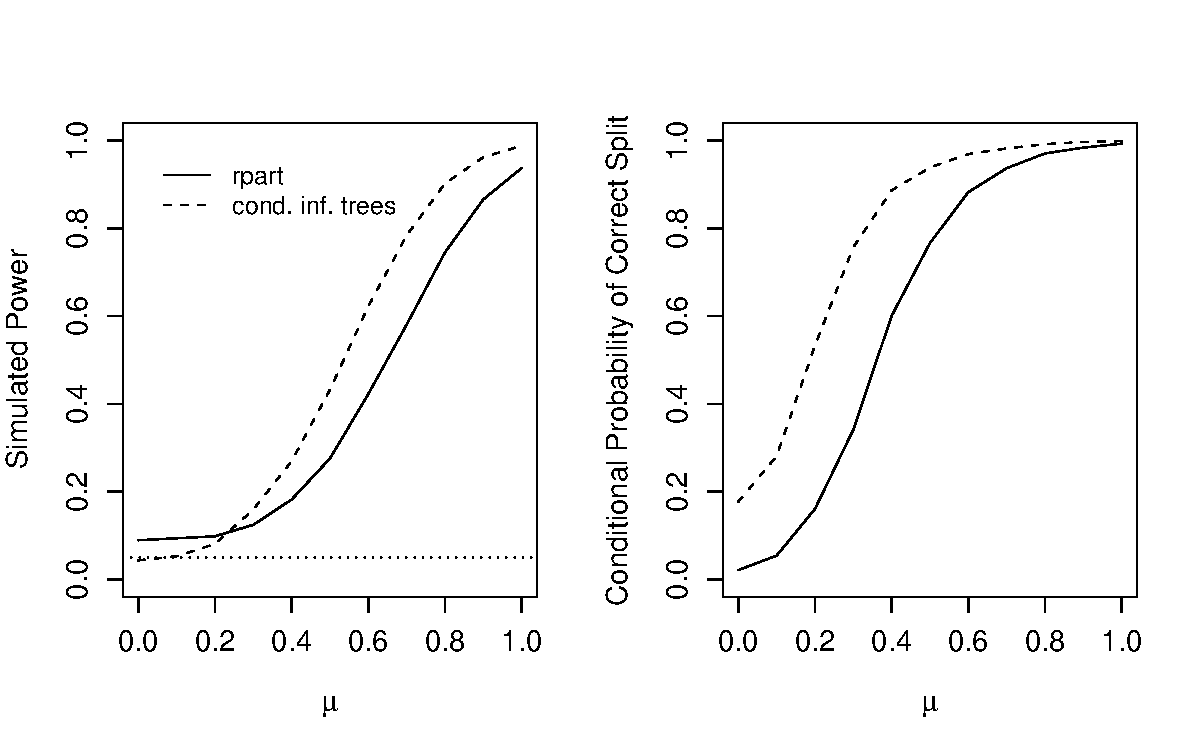
\includegraphics[width = \textwidth]{power_split}
\caption{Simulated power, i.e. the probability of a root split (left), and the simulated
         conditional probability of a correct split in variable $X_6$ given
         that any root split was established (right) are displayed. The 
         dotted horizontal line represents $\alpha = 0.05$.
         The results are based on 10,000 replications. \label{power}}
\end{center}
\end{figure}

The advantageous properties of the conditional inference trees are obvious
for the simple simulation model with one split only. We now extend our
investigations to a simple regression tree with four terminal nodes. The
response variable is normal with mean $\mu$ depending on the covariates as
follows:
\begin{eqnarray} \label{part}
\Y \sim \left\{ \begin{array}{ll} 
             \mathcal{N}(1,1) & \text{if } X_6 = 0 \text{ and } X_1 < 0.5 \\
             \mathcal{N}(2,1) & \text{if } X_6 = 0 \text{ and } X_1 \ge 0.5 \\
             \mathcal{N}(3,1) & \text{if } X_6 = 1 \text{ and } X_2 < 0.5 \\
             \mathcal{N}(4,1) & \text{if } X_6 = 1 \text{ and } X_2 \ge 0.5.
            \end{array} \right.
\end{eqnarray}

We will focus on two closely related criteria describing the partitions
induced by the algorithms: the complexity of the induced partitions and the
structure of the trees. 
The number of terminal nodes of a tree 
is a measure of the complexity of the model and can easily be compared with
the number of cells in the true data partition defined by (\ref{part}). 
However, the appropriate complexity of a tree does not ensure that the
tree structure describes the true data partition well. 
Here, we measure the discrepancy between the true data partition and 
the partitions obtained from recursive partitioning by the
normalized mutual information \citep[`NMI', ][]{StrehlGhosh2002}, essentially
the mutual information of two partitions standardized by the
entropy of both partitions. Values near one indicate similar to equal   
partitions while values near zero are obtained for structurally different
partitions.

For 1,000 learning samples of size $n = 100$ drawn from the simple tree model,
Table \ref{nodes} gives the cross-tabulated
number of terminal nodes of conditional inference trees and pruned
exhaustive search trees computed by \texttt{rpart}. The null hypothesis of
marginal homogeneity for ordered variables \citep{Agresti2002} 
can be rejected ($P\text{-value} <
0.0001$) indicating that the partitions obtained from both algorithms differ
with respect to the number of terminal nodes.
Conditional inference trees select a right-sized tree (four
terminal nodes) in $78.7\%$ of the cases while \texttt{rpart} generates
trees with four terminal nodes for $63.7\%$ of the learning samples. 
In general, pruning as
implemented in \texttt{rpart} tends to produce trees with a larger number of
terminal nodes in this example. 

\begin{table}
\begin{center}
\begin{tabular}{lrrrrrrr|r}
      & \multicolumn{6}{r}{Conditional Inference Trees} & \\
& & 2 & 3 & 4 & 5 & 6 & $\ge$ 7 & \\
& 2 & 3 & 4 & 5 & 0 & 0 & 0 & 12 \\
& 3 & 0 & 48 & 47 & 3 & 0 & 0 & 98 \\
\texttt{rpart} & 4 & 0 & 36 & 549 & 49 & 3 & 0 & 637 \\
& 5 & 0 & 12 & 134 & 25 & 1 & 0 & 172 \\
& 6 & 2 & 6 & 42 & 10 & 1 & 0 & 61 \\
& $\ge$ 7 & 0 & 3 & 10 & 6 & 1 & 0 & 20 \\ \hline
 &  & 5 & 109 & 787 & 93 & 6 & 0 & 1000 \\
\end{tabular}
\caption{Number of terminal nodes for \texttt{rpart} and conditional
         inference trees when the learning sample is actually partitioned into four
         cells. \label{nodes}}
\end{center}
\end{table}

The correct tree structure with four leaves, with the first split in $X_6$ and splits in
$X_1$ and $X_2$ in the left or right node, is detected by \texttt{rpart} in
$63.3\%$ of the simulation runs and in $77.5\%$ of the cases by conditional
inference trees. The NMI measure between the true partition of the data given by (\ref{part})
and the partitions induced by the tree algorithms needs to be compared for
instances with informative NMI measures only, i.e., the cases
where the NMI between \texttt{rpart} and the true data partition and the NMI
between conditional inference trees and the true data partition coincide do
not cover any information. A
density estimate of the NMI difference between partitions obtained from
\texttt{rpart} and
conditional inference tree partitions in Figure \ref{density} shows that the
partitions induced by conditional inference trees are, one average, closer
to the true data partition. 

\begin{figure}[t]
\begin{center}
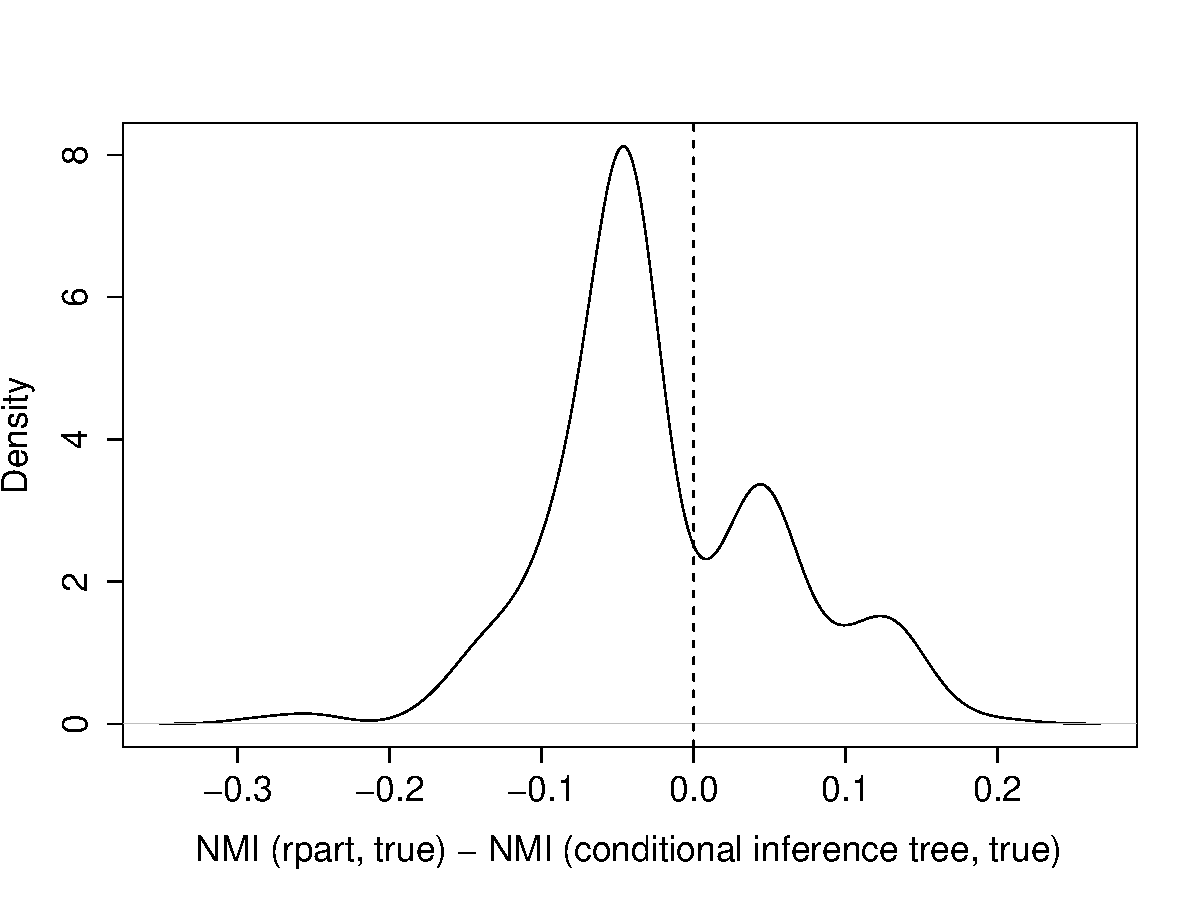
\includegraphics[width = \textwidth]{nmisim}
\caption{Density estimate of the difference in normalized mutual information
         of the true partition and the partitions induced by \texttt{rpart}
         and conditional inference trees. Instances with a NMI difference of
         zero were excluded -- the results are based on $394$ 
         replications. \label{density}}
\end{center}
\end{figure}


\paragraph{Prediction Accuracy.}

Assertion 3) is investigated by means of $11$ benchmarking problems from
the UCI repository \citep{Blake+Merz:1998} as well as the glaucoma data (see
Section \ref{illustrations}).
Characteristics of the problems are given in Table~\ref{benchdata}. We draw
$500$ random samples from the out-of-bag performance measures
(misclassification or mean-squared error) in a dependent $K$-sample design
as described in the conceptual framework for benchmark experiments of 
\cite{Benchmarking2005}. 

\begin{table}[t]
\begin{center}
\begin{tabular}{lrrrrrrr}
               & $J$ & $n$   & NA  & $m$  & nominal & ordinal & continuous \\ \hline
Boston Housing & -- & 506 & --  & 13 & --       & --       & 13    \\
Ozone          & -- & 361 & 158 & 12 & 3      & --       & 9     \\
Servo          & -- & 167 & --  & 4  & 4       & --       & -- \\ \hline
Breast Cancer  & 2 & 699 & 16 & 9  & 4       & 5       & --     \\
Diabetes       & 2 & 768 & --  & 8  & --       & --       & 8     \\
Glass          & 6 & 214 & --  & 9  & --       & --       & 9     \\
Glaucoma       & 2 & 196 & --  & 62 & --       & --       & 62    \\
Ionosphere     & 2 & 351 & --  & 33 & 1       & --       & 32    \\
Sonar          & 2 & 208 & --  & 60 & --       & --       & 60    \\
Soybean        & 19 & 683 & 121 & 35 & 35    & 5       & --     \\
Vehicle        & 4  & 846 & -- & 19 & --       & --       & 19    \\
Vowel          & 11 & 990 & -- & 10 & 1       & --       & 9     \\
\end{tabular}
\caption{Summary of the benchmarking problems showing the number of classes
of a nominal response $J$ (`--' indicates a continuous response), the number
of observations $n$, the number of observations 
with at least one missing value (NA) as well as the measurement
scale and number $m$ of the covariates. \label{benchdata}}
\end{center}
\end{table}


The performance of conditional inference trees is compared to the
performance of exhaustive search trees with pruning (as implemented in
\texttt{rpart}) and unbiased \texttt{QUEST} trees (nominal responses) and
piecewise constant \texttt{GUIDE} trees (numeric responses), respectively.
The tree sizes for \texttt{QUEST} and \texttt{GUIDE} are determined by
pruning as well.

Two performance distributions are said to be equivalent when 
the performance of the conditional inference trees compared 
to the performance of one competitor (\texttt{rpart}, \texttt{QUEST} or \texttt{GUIDE}) 
does not differ 
by an amount of more than $10\%$. The null hypothesis of non-equivalent performances 
is then defined in terms of the ratio of the expectations of the performance
distribution of conditional inference trees and its competitors. 
Equivalence can be established at level $\alpha$ based on two one-sided level
$\alpha$ tests by the intersection-union principle \citep{BergerHsu1996}.
Here, this corresponds to a rejection of the null hypothesis of
non-equivalence performances at the $5\%$ level when the $90\%$ two-sided
\cite{Fieller1940} confidence interval 
for the ratio of the performance expectations is completely included in the 
equivalence range $(0.9, 1.1)$.

%%The distribution of the performance ratios between conditional inference
%%trees and \texttt{rpart} trees together with the Fieller confidence intervals are
%%depicted in Figure~\ref{ratiofig}. The corresponding plot for the comparison
%%of conditional inference trees and \texttt{QUEST}/\texttt{GUIDE} is given in
%%Figure \ref{ratiofigQG}.

\begin{figure}[t]
\begin{center}
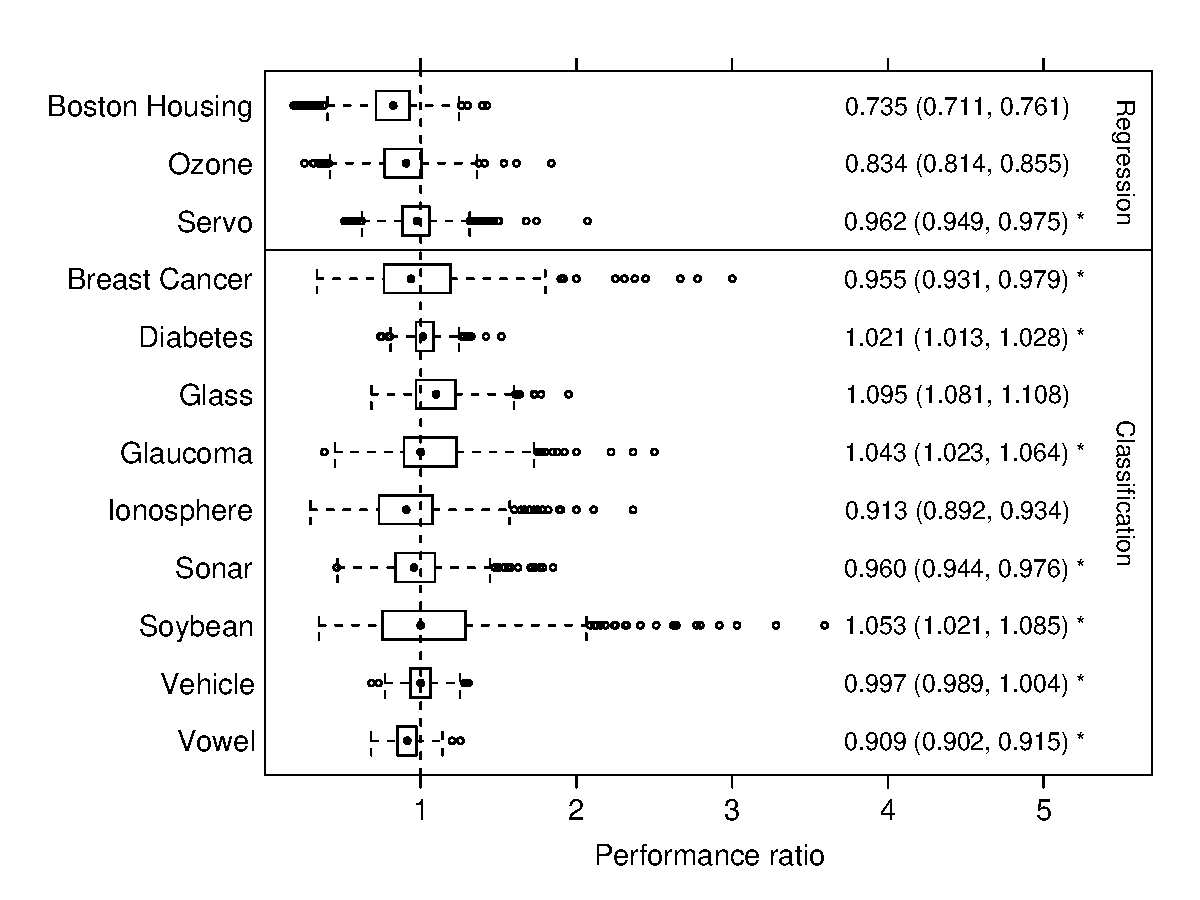
\includegraphics[width = \textwidth]{ratiobox}
%Z%  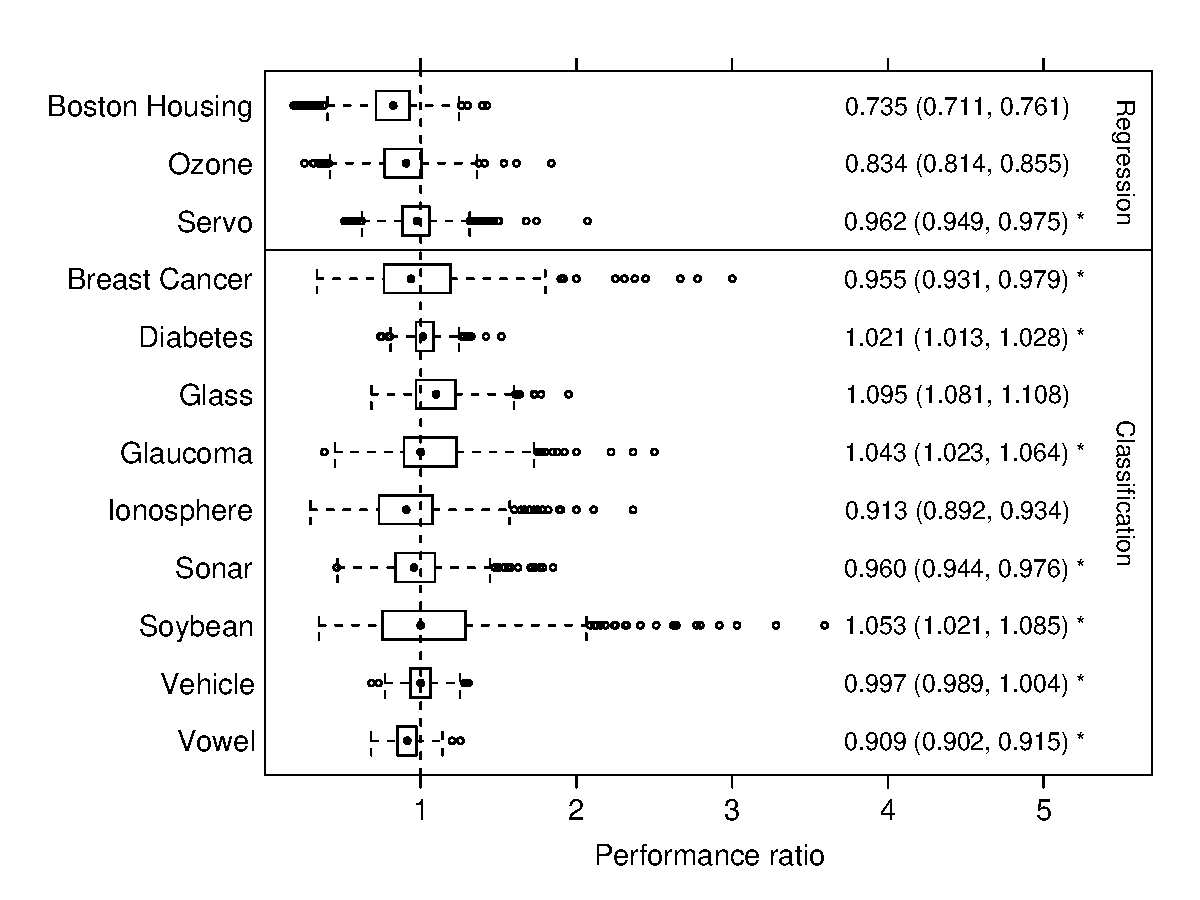
\includegraphics[width = 14cm]{ratiobox}
\caption{Distribution of the pairwise ratios of the performances of the
         conditional inference trees and
         \texttt{rpart} accomplished by estimates and $90\%$ Fieller confidence intervals for
         the ratio of the expectations of the performance distributions. 
         Stars indicate equivalent performances, i.e., the confidence interval 
         is covered by the equivalence range $(0.9, 1.1)$.\label{ratiofig}}
\end{center}
\end{figure}

\begin{figure}[t]
\begin{center}
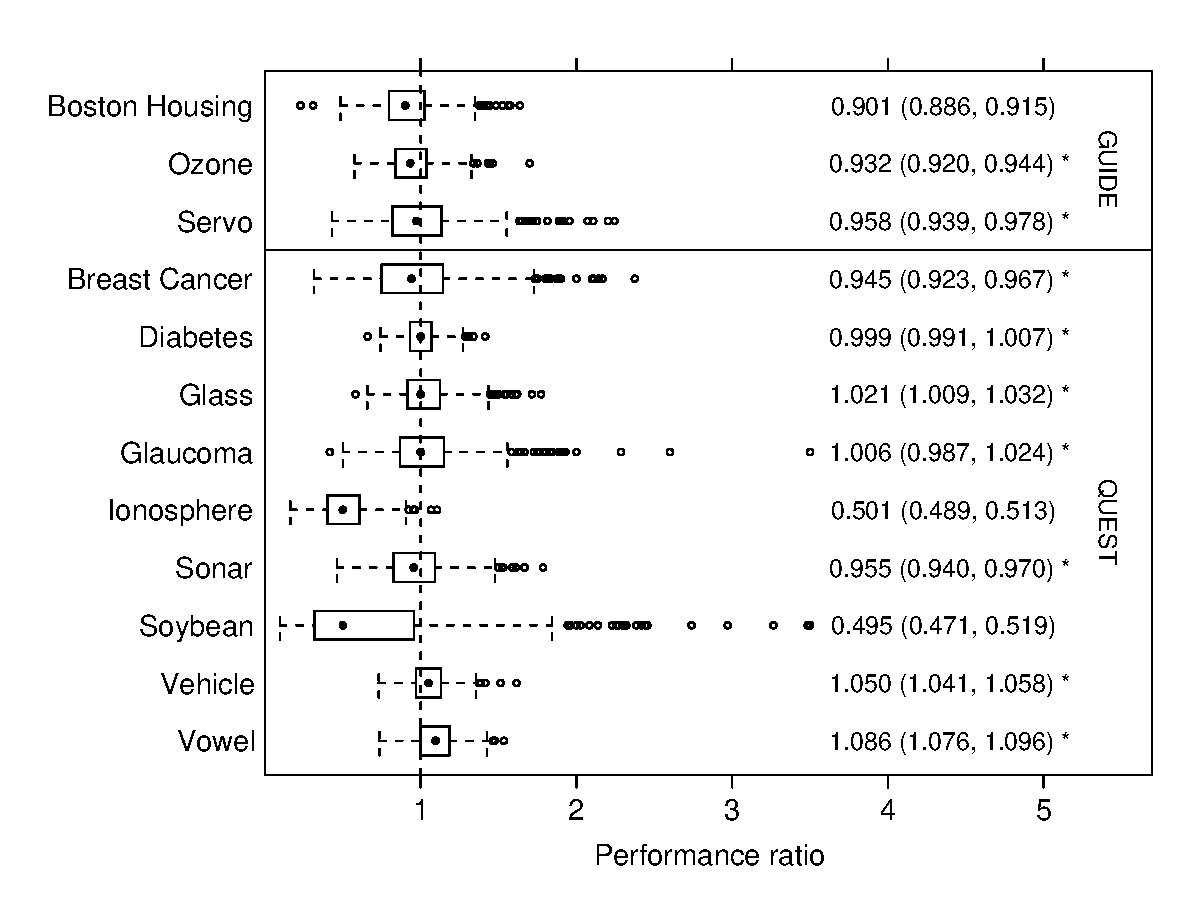
\includegraphics[width = \textwidth]{ratioboxQUEST_GUIDE}
\caption{Distribution of the pairwise ratios of the performances of the
         conditional inference trees and
         \texttt{QUEST} (classification) or \texttt{GUIDE} (regression) 
         accomplished by estimates and $90\%$ Fieller confidence intervals for
         the ratio of the expectations of the performance distributions. 
         Stars indicate equivalent performances, i.e., the confidence interval 
         is covered by the equivalence range $(0.9, 1.1)$.\label{ratiofigQG}}
\end{center}
\end{figure}


The boxplots of the pairwise ratios of the performance measure evaluated for
conditional inference trees and pruned exhaustive search trees
(\texttt{rpart}, Figure \ref{ratiofig}) and pruned unbiased trees 
(\texttt{QUEST}/\texttt{GUIDE}, Figure \ref{ratiofigQG}) are accomplished by
estimates of the ratio of the expected performances and corresponding
Fieller confidence intervals. For example, an estimate of the ratio 
of the misclassification errors 
of \texttt{rpart} and conditional inference trees for the glaucoma data of
$1.043$ means that the misclassification error of conditional inference
trees is $4.3\%$ larger than the misclassification error of \texttt{rpart}.
The confidence interval of $(1.023, 1.064)$ leads to the conclusion that
this inferiority is within the pre-defined equivalence margin of
$\pm 10\%$ and thus the performance of conditional inference trees is on par
with the performance of \texttt{rpart} for the glaucoma data.

\begin{figure}[t]
\begin{center}
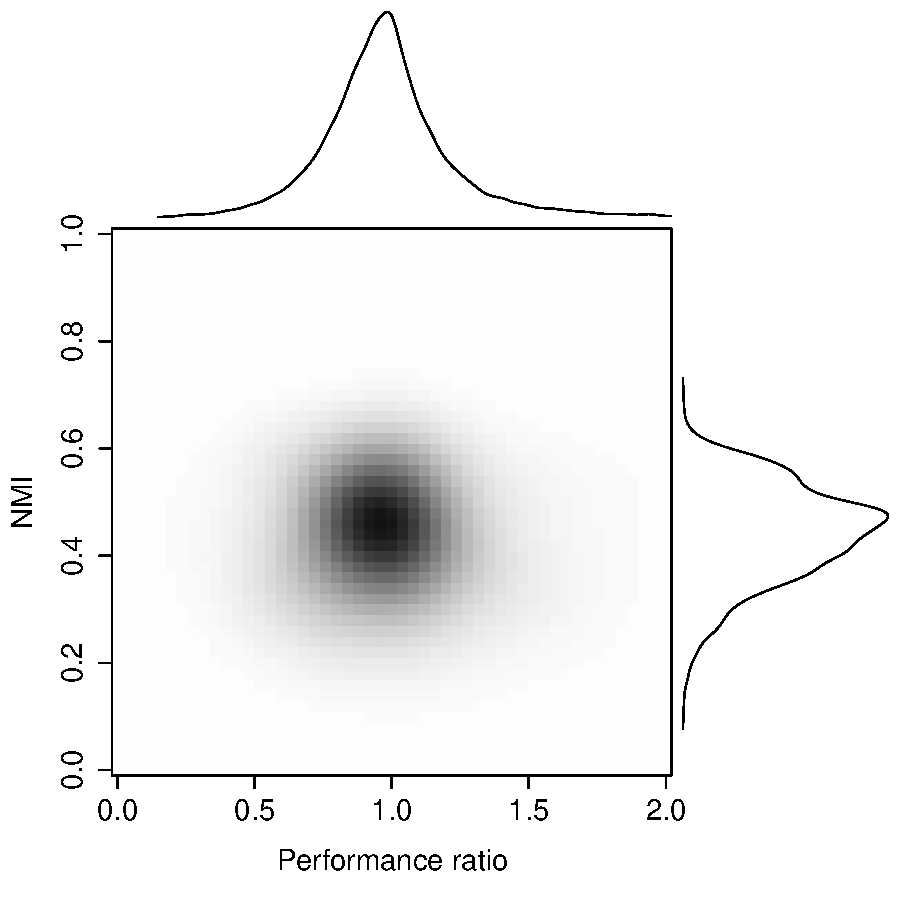
\includegraphics[width = 12cm]{nmiratiodens}
\caption{Distribution of the pairwise performance ratios of conditional
         inference trees and \texttt{rpart} and the normalized mutual
         information measuring the discrepancy of the induced partitions. 
         \label{densfig}}
\end{center}
\end{figure}


Equivalent performance between conditional inference trees and
\texttt{rpart} cannot be postulated for the Glass data. The
performance of the conditional inference trees is
roughly $10\%$ worse compared with \texttt{rpart}. In all other cases, the
performance of conditional inference trees is better than or equivalent to the
performance of exhaustive search (\texttt{rpart}) and unbiased procedures
(\texttt{QUEST} or \texttt{GUIDE}) with pruning.
The conditional inference trees 
perform better compared to \texttt{rpart} trees by a magnitude of $25\%$ (Boston
Housing), $10\%$ (Ionosphere) and $15\%$ (Ozone). The improvement upon
unbiased \texttt{QUEST} and piecewise constant \texttt{GUIDE} models 
is $10\%$ for the Boston Housing data and $50\%$ for the
Ionosphere and Soybean data.
For all other problems, the performance of conditional inference trees 
fitted within a permutation testing framework can
be assumed to be equivalent to the performance of all three competitors. 

The simulation experiments with model (\ref{part}) presented in the first
paragraph on estimation accuracy lead to the impression
that the partitions induced by \texttt{rpart} trees are structurally
different from the partition induced by conditional inference trees. Because
the `true' partition is unknown for the datasets used here, we
compare the partitions obtained from conditional inference trees and
\texttt{rpart} by their normalized mutual information.
The median normalized mutual information is  
$0.447$ and a bivariate density estimate depicted in
Figure~\ref{densfig} does not indicate any relationship between the ratio of
the performances and the discrepancy of the partitions. 

This results is interesting from a practical point of view. 
It implies that two recursive partitioning
algorithms can achieve the same prediction accuracy but, at the same time,
represent structurally different regression relationships, i.e., 
different models and thus may lead to different conclusions about the 
influence of certain covariates on the response.



\begin{center}
\section{DISCUSSION}
\end{center}

In this paper, recursive binary partitioning with piecewise constant fits, 
a popular tool for regression analysis, is
embedded into a well-defined framework of conditional inference
procedures. Both the overfitting and variable selection problems induced by a
recursive fitting procedure are solved by the application of the 
appropriate statistical test procedures to both variable selection and
stopping. Therefore, the conditional inference trees suggested
in this paper are not just heuristics but non-parametric models with 
well-defined theoretical background. The methodology is generally applicable to
regression problems with arbitrary measurement scales of responses and
covariates.
%%To our knowledge, there exist only two approaches for recursive binary partitioning 
%%for ordinal regression. \cite{classifica:1984} introduce the `ordered twoing' 
%%criterion (p.~108) and some implementations of `CHAID' are able to deal with 
%%ordinal response variables. Here, the conditional distribution of linear
%%statistics appropriate for ordinal variables, for example the statistic 
%%of the linear-by-linear association test, is the basis of a non-parametric
%%approach extending the toolbox of ordinal regression models described by
%%\cite{KauermannTutz2003}.
In addition to its advantageous statistical properties, 
our framework is computationally attractive since we do not need to
evaluate all $2^{K-1} - 1$ possible splits of a nominal covariate at $K$
levels for the variable selection.
%% -> Section 3 "Computational Complexity"
%%The computational complexity of the algorithm is of order $n$ and, 
%%for nominal covariates measured at $K$ levels, the evaluation of all
%%$2^{K-1} - 1$ possible splits is not necessary for the variable selection.
In contrast to algorithms incorporating pruning based on 
resampling, the models suggested here can be fitted deterministically, 
provided that the exact conditional distribution is not approximated by
Monte-Carlo methods. 
%% -> Section 3, "Splitting Criteria"
%%Although we restricted ourselves to binary splits, the incorporation of
%%multiway splits in step 2 of the algorithm is possible, for example 
%%utilizing the work of \cite{OBrien2004}.


The simulation and benchmarking experiments in Section~\ref{ec} support two
conclusions: Conditional inference trees as suggested in this paper select
variables in an unbiased way and the partitions induced by this recursive
partitioning algorithm are not affected by overfitting. Even in a very
simple simulation model, the partitions obtained from conditional inference
trees are, on average, closer to the true data partition compared to
partitions obtained from an exhaustive search procedure with pruning. 
When the response is independent of all covariates, the
proportion of incorrect decisions in the root node 
is limited by $\alpha$ and when the response is
associated with one of the covariates, conditional inference trees select
the correct covariate more often than the exhaustive search procedure.
In the light of these findings, the conditional inference trees seem to be
more appropriate for diagnostic purposes than exhaustive search procedures. 
The results of
the benchmarking experiments with real data show that the prediction
accuracy of conditional inference trees is competitive with the
prediction accuracy of both an exhaustive search procedure 
(\texttt{rpart}) and unbiased recursive partitioning (\texttt{QUEST}/\texttt{GUIDE})
which select the tree size by pruning. 
Therefore, our findings
contradict the common opinion that pruning procedures outperform algorithms
with internal stopping with respect to prediction accuracy. 
%%While we are
%%confident that 
%%the difference between the performance of conditional inference 
%%trees and \texttt{rpart} 
%%is due to the variable selection bias of the latter one, the superiority
%%of conditional inference trees compared to the other unbiased procedures cannot
%%be explained this way. 
From our point of view, internal stopping criteria based on hypothesis tests 
evaluated earlier \citep[see for example the results of][]{FrankWitten1998} suffer from 
that fact that the data are transformed in order to fit the requirements of
a certain test procedure, such as categorizing continuous variables for a
$\chi^2$ test,
%%(for example CHAID or GUIDE)
instead of choosing 
a test procedure defined for the original measurement scale of the
covariates.
%%(conditional inference trees).
%%Conditional inference trees are free of any assumptions regarding the distributional 
%%properties of the responses or covariates. 
%% In contrast, `FACT' and most of its successors rely on
%% test procedures bound to classical normal theory.

When the parameter $\alpha$ is interpreted as a pre-defined nominal level of
the permutation tests performed in every node of the tree, the tree
structures visualized in a way
similar to Figures~\ref{glaucoma}--\ref{mammoexp} are valid in a sense that
covariates without association to the response appear in a node only with a
probability not exceeding $\alpha$.  
Moreover, subject matter scientists are most likely more familiar with
the interpretation of $\alpha$ as pre-defined nominal level
of hypothesis tests rather than as a fine-tuned hyper parameter.
Although it is possible to choose
$\alpha$ in a data-dependent way when prediction accuracy is the main focus, 
the empirical experiments in Section
\ref{ec} show that the classical convention of $\alpha = 0.05$ performs
well compared to tree models optimizing the prediction accuracy directly. 
However, while the predictions obtained from
conditional inference trees are as good as the predictions of pruned
exhaustive search trees,
the partitions induced by both algorithms differ structurally. 
Therefore,
the interpretations obtained from conditional inference trees and trees
fitted by an exhaustive search without bias correction cannot be 
assumed to be equivalent. Thus, two rather different partitions, and
therefore models, may have equal prediction accuracy.
Since a key reason for the popularity of 
tree based methods
stems from their ability to represent the estimated regression relationship
in an intuitive way, interpretations drawn 
from regression trees must be taken with a grain of salt.

In summary, this paper introduces a statistical approach to recursive
partitioning. Formal hypothesis tests for both variable
selection and stopping criterion are established. This choice leads to 
tree structured regression models for all kinds of regression problems,
including models for censored, ordinal or multivariate response variables.
Because well-known concepts are the basis of variable selection and 
stopping criterion, the resulting models are easier to communicate to practitioners. 
Simulation and benchmark experiments indicate that conditional inference
trees are well-suited for both explanation and prediction.

%%Nevertheless, one should keep in mind that regression models
%%based on univariate rectangular splits can only serve as a rough
%%approximation to reality. Tree algorithms able to fit non-constant models in
%%terminal nodes (e.g. GUIDE) 
%%provide more flexibility. However, if prediction accuracy is
%%the main target the data analyst aims at, 
%%recursive partitioning procedures are
%%ruled out by much more accurate predictors like some form of ensemble
%%learning or support vector machines anyway.



\section*{ACKNOWLEDGEMENTS}

We would like to thank three anonymous referees, one associate editor and
the editor of JCGS for their valuable comments which lead to substantial
improvements. The work of T. Hothorn was supported by Deutsche 
Forschungsgemeinschaft (DFG) under grant HO 3242/1-1. 



\bibliographystyle{jcgs}
\bibliography{conditionaltrees}


\section*{Appendix A}

An equivalent but computational simpler formulation of the linear statistic
for case weights greater than one can be written as follows. Let $\a = (a_1,
\dots, a_{\ws})$, $a_l \in \{1, \dots, n\}, l = 1, \dots, \ws$, denote the
vector of observation indices, with index $i$ occuring $w_i$ times. 
Instead of recycling the $i$th observation $w_i$ times it is sufficient to
implement the index vector $\a$ into the computation of the test statistic
and its expectation and covariance. For one
permutation $\sigma$ of $\{1, \dots, \ws\}$, the linear statistic
(\ref{linstat}) may be written as 
\begin{eqnarray*}
\T_j(\LS, \w) = \vec \left(\sum_{k=1}^{\ws} g_j(X_{ja_k})
           h(\Y_{\sigma(\a)_k}, (\Y_1, \dots, \Y_n))^\top \right) \in \R^{p_jq}
\end{eqnarray*}
now taking case weights greater zero into account.

\section*{Appendix B}

The results shown in Section~\ref{illustrations} are, up to some labelling, 
reproducible using the following \textsf{R} code:

\renewcommand{\baselinestretch}{1}

\begin{Sinput}
library("party")

data("GlaucomaM", package = "ipred")
plot(ctree(Class ~ ., data = GlaucomaM))

data("GBSG2", package = "ipred")  
plot(ctree(Surv(time, cens) ~ ., data = GBSG2))

data("mammoexp", package = "party")
plot(ctree(ME ~ ., data = mammoexp))
\end{Sinput}



\end{document}
